\documentclass[letterpaper]{article}
\usepackage{iccc}

\usepackage{dialogue}

\usepackage{etoolbox}

\makeatletter
\appto{\PreDialogue}{\global\@newlistfalse}
\makeatother

\newcommand{\jc}[1]{\speak{Joe}{#1}}
\newcommand{\aj}[1]{\speak{Anna}{#1}}
\newcommand{\tl}[1]{\speak{Teresa}{#1}}
\newcommand{\cg}[1]{\speak{Christian}{#1}}

\usepackage{censor}
\usepackage{enumitem}
\usepackage{times}
\usepackage{helvet}
\usepackage{courier}
\usepackage[T1]{fontenc}
\usepackage{csquotes}
\usepackage[utf8]{inputenc}
\usepackage[british]{babel}
\usepackage[style=apa,natbib,backend=biber,url=false]{biblatex}
\let\cite\citep
\usepackage[ddmmyyyy]{datetime}
\renewcommand*{\multicitedelim}{\addsemicolon\space}%
\usepackage{xcolor}
\definecolor{light-gray}{gray}{0.97}
% \usepackage[firstpage]{draftwatermark}
% \SetWatermarkColor{light-gray}
% \SetWatermarkText{\shortstack{Draft\\\today\\\currenttime}}
% \SetWatermarkScale{0.75}

\usepackage{tikz}
\usetikzlibrary{quotes,decorations.text}
\usepackage{figures/circle_arcs_setup}

\usepackage[framemethod=tikz]{mdframed}
\mdfsetup{
skipabove=\baselineskip,
skipbelow=\baselineskip,
innertopmargin=3pt,
innerbottommargin=5pt
}

\newcommand*{\sourceatright}[1]{\unskip\hspace{1em plus 1fill}%
\nolinebreak[3]\hspace*{\fill}\mbox{#1}}%LaTeX Hacks 

\usepackage{etoolbox}
\makeatletter
\patchcmd{\@verbatim}
  {\verbatim@font}
  {\verbatim@font\footnotesize}
  {}{}
\makeatother

\usepackage[
  bookmarks=false,
  pdfpagelabels=false,
  hyperfootnotes=false,
  hyperindex=false,
  pageanchor=false,
%  colorlinks,
  hidelinks
]{hyperref}

\DeclareLanguageMapping{british}{british-apa}
% \addbibresource{papers.bib}
\addbibresource{poetryICCC.bib} %

%% \urlstyle{tt}
\AtBeginBibliography{\def\UrlFont{\footnotesize\tt}}
\renewcommand*{\finalnamedelim}{%
  \ifnumgreater{\value{liststop}}{2}{\finalandcomma}{}%
  \addspace\&\&\space\space}
%
\AtEveryCitekey{\renewcommand*{\finalnamedelim}{%
  \ifthenelse{\value{listcount}>\maxprtauth}
    {}
    {\ifthenelse{\value{liststop}>2}
       {\finalandcomma\addspace\bibstring{and}\space}
       {\addspace\bibstring{and}\space}}}}

\AtBeginDocument{\renewcommand*\finalandcomma{\addcomma}}
\AtBeginBibliography{%
  \renewcommand*{\finalnamedelim}{%
    \ifthenelse{\value{listcount}>\maxprtauth}
      {}
      {\finalandcomma\addspace\bibstring{and}\space}}}

% \pdfinfo{
% /Title (Test)
% /Subject (Proceedings of ICCC)
% /Author (ICCC)}
% The file iccc.sty is the style file for ICCC proceedings.

\title{Computational Poetry Workshop: Making Sense of Work in Progress\\[.2cm](A play in one act)}
%% \author{J. Corneli\thanks{Corresponding author. Email: {\tt j.corneli@gold.ac.uk}} \\ Goldsmiths College
%% \And A. Jordanous \\ University of Kent \\
%% \And R. Shepperd \\ Goldsmiths College
%% \And \textbf{M. T. Llano}  \\ Goldsmiths College
%% \AND \textbf{J. Misztal}  \\ Jagiellonian University
%% \And \textbf{S. Colton}  \\ Goldsmiths College
%% \And \textbf{C. Guckelsberger}  \\ Goldsmiths College
%% }
\setcounter{secnumdepth}{0}

\thispagestyle{plain}
\pagestyle{plain}

\begin{document} 
\begin{center}
\textbf{Computational Poetry Workshop: Making Sense of Work in Progress}\\[.2cm](A play in one act)
\end{center}

\bigskip

%\maketitle
%% \begin{abstract}
%% \begin{quote}
%% Creativity cannot exist in a vacuum; it develops through feedback,
%% learning, reflection and social interaction with others. However, this perspective
%% has been relatively under-investigated in computational creativity
%% research, which typically examines systems that operate
%% individually. 
%% % We develop a set of requirements for creativity systems
%% % that can incorporate communication and give and receive
%% % feedback. 
%% % As a thought experiment to test these ideas, 
%% We develop a thought experiment showing how structured dialogues can help develop the
%% creative aspects of computer poetry.
%% Centrally in this approach, we ask questions of a poem, inviting it to tell us in what way it may be considered a ``creative making.''

%% % in what way can CC enhance the human workshop?

%% \medskip

%% \textbf{Keywords}: computer poetry, social creativity, flowcharts, Writer's Workshops
%% \end{quote}
%% \end{abstract}

% Study papers
% These will be papers which draw on allied fields such as psychology, philosophy, cognitive science or mathematics;
% or which appeal to broader areas of Artificial Intelligence and Computer Science in general;
% or which appeal to studies of the field of Computational Creativity as a whole.
% The emphasis here is on presenting enlightening novel perspectives related to the building,
% assessment or deployment of systems ranging from autonomously creative systems to creativity support tools.
% Such perspectives can be presented through a variety of approaches including ethnographical studies,
% thought experiments, comparison with studies of human creativity and surveys.


%% TODO LIST FOR REVISION
% - trim the introduction

%% \begin{mdframed}
%% {\small
%% \vspace{-.3cm}
%% \tableofcontents
%% }
%% \end{mdframed}
%% \newpage

%% \begin{quote}
%% {\small `We \emph{can} talk,' said the Tiger-lily: `when there's anybody worth talking to.'\\
%% \sourceatright{Through the Looking Glass, Lewis Carroll}}
%% \end{quote}



\textbf{Dramatis Personae.}

\smallskip

\begin{tabular}{lp{.7\columnwidth}}
\sc{Joe} & Presenting author \\
\sc{Anna} & Reviewer 1 \\
\sc{Teresa} & Reviewer 2 \\
\sc{Christian} & Workshop moderator \\
\end{tabular}

\bigskip

\section*{Initial backdrop}

\medskip

A picture like this, with the title of our paper above and the names
of authors below:

\medskip

\begin{mdframed}
\begin{center}
\textbf{Computational Poetry Workshop:\\ Making Sense of Work in Progress}


\includegraphics[width=\columnwidth]{boink}

J. Corneli, A. Jordanous, R. Shepperd, M. T. Llano,\\J. Misztal, S. Colton, and C. Guckelsberger

\end{center}
\end{mdframed}

\medskip


\section*{Scene 1}

\begin{dialogue}
\direct{The workshop participants have gathered to discuss the paper
  ``Computational Poetry Workshop: Making Sense of Work in Progress.''}

\smallskip

\cg{If you could move these chairs together in a sort of circle\ldots}

\direct{They move the chairs into more of a semi-circle, so that the
  audience can see them too.}

\aj{If we can all see each other that should be fine.}

\cg{I guess you've all had a chance to read the paper already?}

\direct{The reviewers nod and say ``yeah.''}

\cg{Joe, could you give us a quick summary and highlight the things
  you're most interested in getting feedback about?  I guess, given
  the content of the paper, you're pretty much familiar with the way
  this sort of thing works, but, just to be clear, once you're done
  with that quick presentation, we'll give you feedback, and you
  should just take notes. OK?}

\end{dialogue}

\newpage

\begin{dialogue}
\direct{As \refer{Joe} speaks, the pieces of text in italics appear
  one by one as bullet points on a single slide behind the authors.
  That slide stays on screen throughout the rest of Scene 1.}

\begin{mdframed}
\begin{itemize}
\item \emph{How has the social dimension of creativity been
  explored in CC to date?}
\item \emph{Let's give artefacts more agency, design computer programs
  with more autonomy, and focus research effort on understanding
  creative evolution.}
\item \emph{Let's ask: ``How a created artefact can tell us about its own
  making?''}
\item \emph{A theory of poetics rooted in the making of
  boundary-crossing objects and processes.}
\item \emph{The paper is claiming that workshops are suitable
  environments for autonomous learning and development of the creative
  process.}
\end{itemize}
\end{mdframed}

\jc{Sure.  OK, so, the paper is called ``Computational Poetry
  Workshop: Making Sense of Work in Progress.''  It's for ICCC'15, the
  International Conference on Computational Creativity.  It's already
  been accepted for publication but I want to improve it so that it's
  a bit more clear, since the reviewers expressed some doubts.  The
  paper starts out by looking at \emph{how the social dimension of
    creativity has been explored in CC to date.}  It basically says
  that the ideas of social interaction, feedback, and evaluation have
  frequently been discussed in CC, but that implementation and
  theorisation around these topics have been more limited.  It then
  goes on to suggest that we what should do is \emph{give artefacts
    more agency, design computer programs with more autonomy, and
    focus research effort on understanding creative evolution.}  I
  want to check with you if that part is clear, because the
  perspective isn't exactly traditional.  The underlying idea is much
  more broadly applicable than CC, and it asks: \emph{``How a created
    artefact can tell us about its own making?''}  The paper takes
  this idea and runs with it a bit, to suggest that in principle
  computers can engage in dialogue, with, and about, poems.  Out of this comes the
  more profound idea of \emph{a theory of poetics rooted in the making
    of boundary-crossing objects and processes.}  That sounds a bit
  abstract, so I want to make sure it's coming across well.  After
  presenting these more theoretical ideas, the paper makes some
  initial steps towards a computational simulation.  It develops a
  thought experiment that imagines an improved version of the FloWr system
  that's being developed in the CCG group at Goldsmiths being used
  to run ``writers workshops'' for computer poetry.  There are lots of
  technical facilities that could make that easier, but the main thing
  I want to get feedback from you on today is what you think about the
  core idea of the workshop approach in a computing context.  \emph{The paper is claiming that
    workshops are suitable environments for autonomous learning and
    development of the creative process.}  Finally, it makes some sort
  of political claims about dialogue within CC, but the basic thrust
  here is that we should be getting our computer programs talking to
  each other.  I'm curious to know what you guys think about that.
  And, yeah, that's it.}

\section*{Scene 2}

\direct{The projection switches to a blank screen.  \refer{Joe} takes
  notes on what people are saying, and these notes accumulate on the
  screen.  The notes should resemble a poem by the end of the scene.}

\cg{Thanks Joe.  Does anyone want to sum up what they think the paper
  is about? \direct{Looks around.}  I guess I'll start.  The paper
  studies how social interaction through dialogue can be applied to
  computational creativity processes.  It uses poetry generation as an
  example and aims to develop a ``thought experiment'' in this
  domain.}

\tl{I'd say it's basically a study about how to use social creativity
  to generate poems. The proposal consists on using the Writer’s
  Workshop model to maintain a dialogue between different poetry
  generators and poetry critics in order to improve the final poem.
  In the paper, there are presented different questions that could be
  asked by a person when reading a poem, and the questions that a
  computer could ask.  Then, the results are compared.  Finally, the
  proposal is applied showing a hypothetical adapted design of the
  FloWr system with a human critic and a poetry generator.}

\cg{Thanks Teresa, I think that's a good summary.  You're right, the
  questions that people and computers can ask form a pretty central
  part of the paper.  Maybe that has to do with the ``theory of
  poetics that is rooted in the making of boundary-crossing objects
  and processes'' although frankly that's still pretty abstract for
  me.  Anna, what do you think?  What does the paper accomplish?}

\aj{Well, first of all, I think this paper makes a reasonable start
  toward describing a workshop-style collaboration on writing (and
  reading) poetry.  It does only preliminary work toward this, but
  raises a lot of interesting questions.  For example, it made me
  wonder how a workshop approach differs from more traditional peer
  review -- if at all?  Like Teresa said, it seems like the paper is
  making the case that the workshop is not just useful for reviewing
  things after they're created but for helping create them in the
  first place.  Although there is some interesting tension there.  If
  the emphasis is on poetry generation it would probably be useful to
  include a more thorough review of systems like Slant (by Montfort,
  P\'erez y P\'erez and Harrell), which is a blackboard-based
  multi-agent system.  But I can see that the workshop idea is a bit
  different from more traditional multi-agent systems like that one.}

\tl{I think it's really nice to see the discussion of process as the
  content of a poem, not because everyone would agree that this is
  correct but because it asserts a particular, deliberate perspective
  on poetry.  Christian, I think what the philosophical ideas are
  saying is that the poem is a sort of dialogue that the reader gets
  involved with -- but I agree that could be said a lot more simply.
  Another thing is that the way in which the agency is split up on
  page 4 (a separate counting agent and breathing agent) of course
  does not represent the different perspectives of workshop
  participants.  A workshop where everyone has the same sort of
  expertise, along these lines, could be successful as a computer
  program.  But if it is very culturally homogeneous, it's not going
  to say anything very interesting.  My question is how this model can
  include cultural and idiosyncratic differences in ways that are
  given first-order representations, given how important those
  differences are.}

\cg{OK. Now I think we're getting into the question ``What could be
  improved about the paper?''  So, what do you think about that?}

\tl{To be honest, it is sometimes difficult to read.  I also think a
  better example with more participants could be useful to understand
  the proposal.  In fact, at some point quite a few more examples and
  experiments will really be needed, to really evaluate the proposal,
  but I understand that the current version is a study paper rather
  than a technical paper.}

\aj{Following on from what Teresa said, my only concern here is that
  too little has been done in terms of modeling and system-building
  for others to effectively build upon, or argue for or against the
  applicability of this kind of design in a computing context.  If you
  want to be more computationally convincing without building a
  concrete implementation, I was thinking you could break the process
  into phases like these: \direct{\refer{Anna} refers to her notes,
    and indicates each step clearly, with a gesture or number;
    \refer{Joe} should make sure to capture each of these points in
    his on-screen notes.} \direct{1} Building a model of the text,
  \direct{2} Tagging elements of interest, \direct{3} Generating
  feedback based on assocations drawn between these elements,
  \direct{4} Asking for more information to understand the feedback,
  \direct{5} Creating rationale for the feedback and, on the part of
  the author, \direct{6} Updating the point of view.  To be honest,
  any one of those steps could probably be a PhD project, but with a
  division of labour like that, it starts to look more computationally
  feasible.}

\cg{I also find it a bit hard to see the computational focus in the
  current paper, although maybe that's because it's doing double duty
  as a kind of manifesto.  I think it is certainly presenting a very
  interesting challenge and food for thought for later discussion and
  more precise elaboration.  Oh, and there are also a few typos, I can
  pass you a list. Any other comments?}

\direct{Looks around, but people are signalling they're done.}

\cg{Joe, do you have any questions about the discussion so far?}

\jc{\direct{A bit hurt because he's imagining the philosophical ideas
    haven't come across very well.}  No, thanks, I think that's all
  pretty clear.}

\cg{I think there's a lot there, but -- if I can make a final summary
  comment -- I think it would be good if the work was presented with
  some more structure.  If not in the paper itself, then at the
  conference: a well structured and concrete presentation, perhaps
  following an example that looks into the role of different agents
  could help spark the discussion.  \direct{Breaking the 4th wall.}
  With that, let's take some questions and comments from the
  audience.}

\bigskip

\direct{(Possible) Applause, and Q\&A.}

\end{dialogue}
%% \section{Introduction}
\label{sec:intro}

% \begin{itemize}
% \item Why poetry?
% \item Why FloWr?
% \item Why Workshop?
% \end{itemize}

We are writing in a large part to champion Alan Turing's
proposal that intelligent machines should ``be able to converse with
each other to sharpen their wits'' \cite{turing-intelligent}. 
%
The formalism that we propose builds on the notion of social cybernetics that flows
from the following propositions of Heinz von Foerster's, which he uses to theorise systems
in which participants can responsibly specify their own roles in relationship to
other system participants:

\begin{quote}
``Anything said is said \emph{by} an observer.'' \\
``Anything said is said \emph{to} an observer.''\\
\sourceatright{\cite{von2003cybernetics}}
\end{quote}

According to Jaako Seikkula and Tom Arnkil, who draw on the philosophical and literary analysis of Mikhail Bakhtin \cite{bakhtin2010toward,bakhtin1984problems} in their approach to psychosocial work,
\begin{quote}
``Dialogues could be called `the art of crossing boundaries'.  Instead of trying to control others, the parties reach out towards each other to hear their views better, to generate shared languages and to join resources.''
\sourceatright{\cite[p. 23]{seikkula2014open}}
\end{quote}

This paper outlines a study of social creativity with a dialogical emphasis, taking computer
poetry as our working domain.  It uses the Writer's Workshop model
\cite{gabriel2002writer} as the virtual laboratory in which to conduct a thought experiment.
The findings of our study are applied to the FloWr system \cite{charnley2014flowr}. 
We focus on the following questions in turn:
%\subsection{Outline}


\begin{itemize}[label=--,itemsep=0pt]
% BACKGROUND
% - a few more details
\item How has the social dimension of creativity been explored in CC to date? 
% PHILOSOPHY AND METHODS
% - break into subsections and add tools, integrate to table
%CG: Modified this to connect rosies methodology to the workshop and CC
\item How can a created artefact tell us about its making, and what can this contribute to CC?
% DESIGN
\item How can computer poetry contribute to developing a process-based theory of poetics? 
% FLOWR
% - Teresa to revise 
\item What would have to change about the FloWr system to implement the computational poetry workshop approach?
% DISCUSSION
% - keep it?
\item What are the pros and cons of the workshop approach?
% CONCLUSIONS
% - taking into account Christian's comment, I've revised this and will edit the conclusion to align.  JC.
\item What might be the future role of dialogue in CC?
\end{itemize}

%%% Not nec. needed
%%% In the background section, we will focus on social creativity in the computational creativity domain and more specifically in computer poetry. This will be followed by a Methods section, in which we ...

%%% Local Variables: 
%%% mode: latex
%%% TeX-master: "poetryICCC"
%%% End: 
 
%% \section{Background}
\label{background}

\subsection{Social creativity in CC}

Although we have adopted the term ``social creativity'' following
\cite{saunders12} and with the specific understanding developed above,
we could also refer in a similar spirit to situated, interactive,
communal, contextual, conversational, group, dialogical,
discourse-based, community-based, interaction-based, or
feedback-informed creativity.

The point is that creativity cannot exist in a vacuum.  The very
essence of creativity lives in its appreciation by the creative entity
themselves and its audience.  As we have remarked elsewhere,
creativity is in the eye of the beholder.  During the creative
process, self-evaluation abilities are crucial
\cite{poincare29,csik88}. Social creativity expands upon this
paradigm by bringing co-creators into the process, and creating works
that rely on dialogue, reflection, and multiple perspectives. The
``results'' may be steeped in process and will not always be based in
consensus.

The Four Ps of creativity -- the creative Person, Product, Process and
Press (i.e. environment) \cite{rhodes61,mackinnon70} -- have been
emphasised in general creativity research.  \emph{Pluralising} these
terms would call attention to a social dimension of creativity, and
leads to a more inclusive and encompassing approach to the study of
creativity -- one that accommodates multiple perspectives. The
Pluralised Ps remind us that it is not sufficient to model a lone
creator or to generate an attractive artefact.  To model creativity
more completely, we also need to consider the environment in which a
creative person operates, and how the environment is used in the
creative process.

Computational creativity research has achieved many successes in
computational generation of creative products. The question of how
these systems could adapt and learn from feedback to improve their
creativity, however, remains underexplored in computational creativity
despite evaluation being a pivotal contributory part of the creative
process. Researchers have generally preferred to take on the task of
generating artefacts that could be seen as creative, as a necessary
prior to the task of incorporating self-evaluation within a creative
system \cite{jordanous11iccc}.

Some notable exceptions exist, highlighting the importance of the
environment in which a creative system is situated \cite{mcgraw93,
  sosa09, perezyperez10MM, pease10, saunders12}, with some of this
work influenced by the DIFI (Domain-Individual-Field-Interaction)
framework \cite{csik88}. Generally, however, social interaction
between creative agents and their audience is an area which has been
neglected. Increased development of the interactivity of creative
systems, especially where this affects the way these systems works, is
pleasing to see and deserves further attention
\cite{coltonwiggins12}.

\begin{mdframed}
\textbf{Other CC material?  Anything about poetry in particular?  It
  might be a good idea to mention Tristan Tzara, Brion Gysin, etc.
  Probably at least a few words about FloWr here as well.}

 E.g. \cite{jordanous10}?  Definitely we should cite
\cite{misztal2014poetry} and explain a bit about the MASTER system.
\end{mdframed}

\subsection{Writer's Workshops}

Quoting \cite[pp. 2--3]{gabriel2002writer}:

\begin{quote}
The original idea behind the writers' workshop was to do a \emph{close
  reading} of a work, to use the term F. R. Leavis coined for the
practice of looking at the words on the page rather than the
intentions of the author or the historical and aesthetic context of
the work.  Under this philosophy, the workshop doesn't care much what
the author feels about what he or she wrote, only what's on the page.
This corresponds to the philosophy of the New Critics, which held that
the work was its own ``being,'' with its own internal consistency and
coherence, which could be studied apart from the author.  Moreover,
this approach is nearly identical to that of the Russian formalists,
who thought that the proper approach to literature was to study how
literary texts actually worked, their structures and devices.
\end{quote}

Framing and any other contextualisation of the work \emph{as it is
  intended to be presented} is permitted, and receives critical attention.

In \cite{serendipity-arxiv}, we described a template for a pattern
language for interactions in a computational poetry workshop, closely
following Gabriel's outline of the relevant steps: {\tt presentation},
{\tt listening}, {\tt feedback}, {\tt questions}, and {\tt
  reflections}.\footnote{To this should be added the potential for
  real-time {\tt replies} by critics to {\tt questions} asked by the
  presenting author, before subsequent ``offline'' {\tt reflections}.}
We used this template to expand several of the patterns of serendipity
described by \cite{van1994anatomy}, showing how they could be used to
foster discovery and invention in a workshop environment.



%%% Local Variables: 
%%% mode: latex
%%% TeX-master: "poetryICCC"
%%% End: 
 
%% \section{Methods}
\label{sec:methods}

%\subsection{Context and process}

\begin{figure}
\resizebox{\columnwidth}{!}{%
%% For final:
\begin{tikzpicture}
%  \draw[thick] (4,0) node[below={2cm}] {\emph{A.~``mere generation''}}
%                     pic[red, -latex]{darc=100:270:1.3cm:Chicken:Lay:2.4cm:3cm}
%                     pic[red, -latex]{uarc=280:450:1.3cm:Egg:Hatch:1cm:.1cm};
%
  \draw[thick] (4.0,0) node[below={2cm},align=center] {\emph{A.~how to become a writer\footnotemark}}
                      pic[red, -latex]{darc=100:270:1.3cm:{}:{Write for 8 hours a day}:1cm:.3cm}
                      pic[red, -latex]{uarc=280:450:1.3cm:{}:{Read for 8 hours a day}:1cm:.3cm};
%
  \draw[thick](8.5,0) node[below={2cm}] {\emph{B.~``the Other''}}
                     pic[red, -latex]{darc=100:270:1.3cm:Statement:Speak:2.1cm:2.6cm}
                     pic[red, -latex]{uarc=280:450:1.3cm:Response:{Listens and interprets}:.2cm:.1cm};

%  \draw[thick] (4,-5.5) node[below={2.2cm}] {\emph{D.~learning by doing}}
%                        pic[red, -latex]{darc=100:240:1.5cm:Poet:Write:3cm:2.7cm}
%                        pic[red, -latex]{rarc=250:320:1.5cm:Poem:Responds:1cm:.5cm}
%                        pic[red, -latex]{uarc=330:450:1.5cm:Context:Speaks:1cm:.1cm};
%
%
  \draw[thick] (13,0) node[below={2cm}] {\emph{C.~proto-workshop}}
                        pic[red, -latex]{larc=100:180:1.3cm:Poet:Writes:1cm:.2cm}
                        pic[red, -latex]{rarc=190:270:1.3cm:Poem:Responds:1cm:.4cm}
                        pic[red, -latex]{rarc=280:360:1.3cm:Context:Speaks:.7cm:.7cm}
                        pic[red, -latex]{larc=370:450:1.3cm:Reader:Responds:.8cm:.2cm};

%  \draw[thick] (13,-5.5) node[below={2.2cm}] {\emph{F.~how computers work}}
%                       pic[red, -latex]{darc=100:180:1.5cm:{}:Print:1.5cm:1.4cm}
%                       pic[red, -latex]{rarc=190:270:1.5cm:{}:Loop:1cm:1.4cm}
%                       pic[red, -latex]{rarc=280:360:1.5cm:{}:Read:1cm:1.4cm}
%                       pic[red, -latex]{larc=370:450:1.5cm:{}:Eval:1.4cm:.2cm};
% Note:
% controls at end: offset of outer text, followed by offset of inner text
\end{tikzpicture}

%% For quick compiling
% 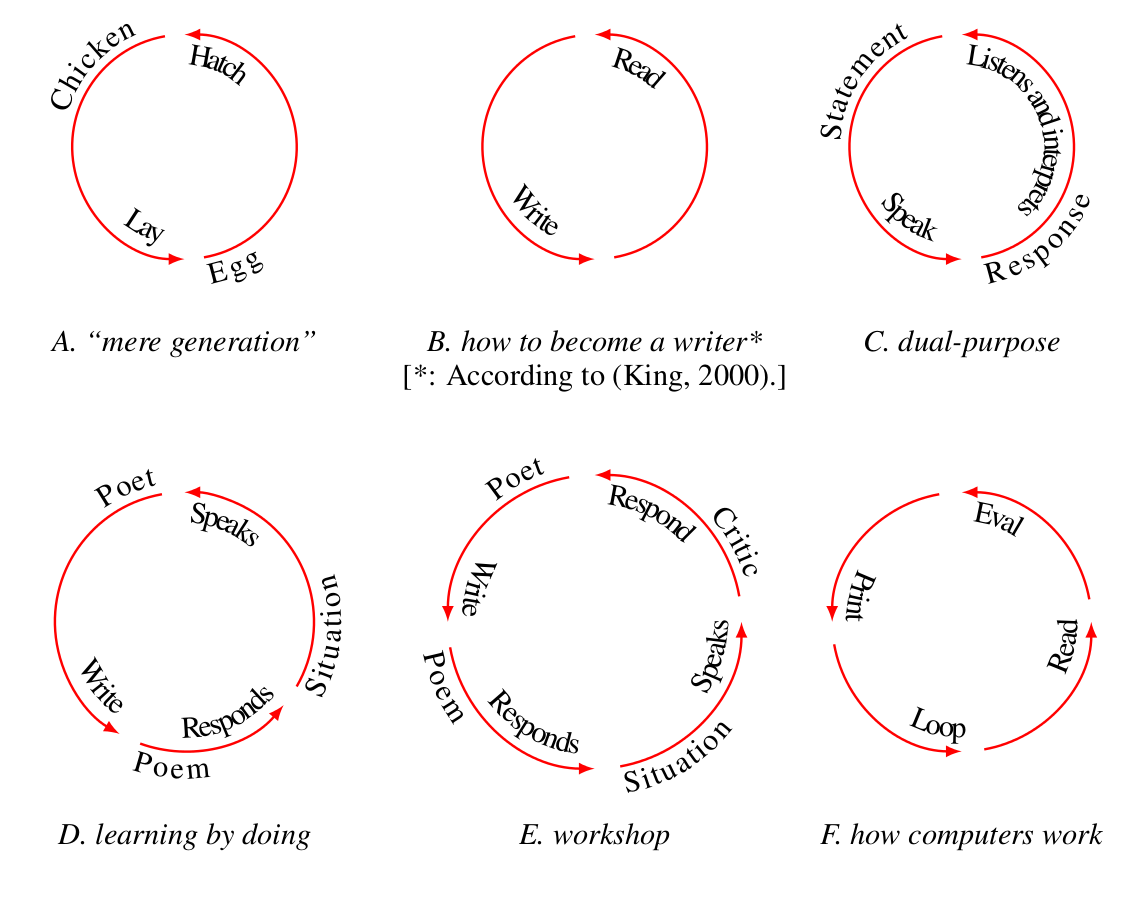
\includegraphics{figures/cycles_shortcut}
}

\caption{(A) gives a simple recipe for the growth and
development of a writer;
(B) \emph{response} always has dimensions that goes beyond the
utterance that is overheard;
(C) adds a \emph{reader} who shares the context with the writer and responds.%, and who responds to this context particularly as it is expressed through the poem
\label{fig:cycles}}
\end{figure}


% Figure \ref{fig:cycles}(A) shows the standard chicken-and-egg problem,
% designed to provoke questions about \emph{evolution};
%%
% 1(B) shows an analogous picture that gives a simple recipe for the growth and
% development of a writer;
%%
% 1(C) is a formally similar diagram that squares up to the metalinguistic features of the situation, showing
% that a \emph{response} (which may be verbal, visceral, physical or
% something else) always has dimensions that goes beyond the utterance that is overheard;
%%
% 1(D) examines in further detail what happens when someone \emph{writes} 
% -- namely, writing as a response to some perceived disturbance, newly identified problem, etc., and writing as it responds to the disturbance does itself become an agent of change;
% Note: we've elided the word "situation" as a totalising concept
%%
% 1(E) adds a \emph{reader} who shares the context with the writer, and who responds to this context particularly as it is expressed through the poem;
% Note: we could call this character a "reader" instead, since "criticism" is pre-judges what they are going to do
% There is another way to read this as related to "crisis" and the different things that can be embedded in
% the poem.
%%
% 1(F) shows that this scenario is not as unfamiliar to computer programmers as it might
% otherwise sound -- consider that the ``Eval'' phase in a
% Read-Eval-Print loop can be interrupted with a debugger to fine-tune
% program operation.

\subsection{``What are the proposed `lab rats'?''}

\footnotetext{According to \citep{king2000writing}.}

% We take as our study of interest the domain of computational poetry. Figure \ref{fig:cycles} illustrates different representations of cyclical processes within creativity, from the simplistic ``mere generation'' through to complex interplays between creator and critic/reader. 

The generative side of the cycles in Figure \ref{fig:cycles} has been studied more than the reflective side.
Our ``lab rats'' are, accordingly, not poems per se, but rather,
\emph{instances of reading and responding to poetry}.  Naturally, such responses could be more or less
``canned'' (as with Michael Cook's humorously nonspecific
AppreciationBot\footnote{\url{https://twitter.com/appreciationbot}}), so the question becomes: what constitutes an
interesting and useful response, and how will these be
developed?  The idea of responses is useful at various levels.
We focus here on staging an encounter between writer and reader.

\subsection{Writer's Workshops}

Quoting \cite[pp. 2--3]{gabriel2002writer}:

\begin{quote}
The original idea behind the writers' workshop was to do a \emph{close
  reading} of a work%, to use the term F. R. Leavis coined for the
%practice of 
... looking at the words on the page rather than the
intentions of the author or the historical and aesthetic context of
the work.  Under this philosophy, the workshop doesn't care much what
the author feels about what he or she wrote, only what's on the page.
%This corresponds to the philosophy of the New Critics, which held that
%the work was its own ``being,'' with its own internal consistency and
%coherence, which could be studied apart from the author.  Moreover,
%this approach is nearly identical to that of the Russian formalists,
%who thought that the proper approach to literature was to study how
%literary texts actually worked, their structures and devices.
\end{quote}

Framing and any other contextualisation of the work \emph{as it is intended to be presented} is permitted, and receives critical attention.
% we described a template for a pattern
% language for interactions in a computational poetry workshop, closely
We define a \emph{Workshop} closely following
Gabriel's outline, to be an activity consisting of these steps:
%itemize?
{\tt presentation}, {\tt listening}, {\tt feedback}, {\tt questions}, and 
 {\tt reflections}.  The first and most important feature of {\tt feedback} is
 for the listener to say what they heard; in other words, what, for them, is in the work.  In some
 settings this is augmented with {\tt suggestions}.  After any
 {\tt questions} from the author, the commentators may make {\tt replies} to offer clarification. 
In  \cite{feedback-arxiv} we used the Workshop framework 
to expand several patterns of serendipity described by
\cite{van1994anatomy}, showing how they could be used to foster discovery
and invention in a social context.

%%%%%%%%%%%%%%%%%%%%%%%%%%%%%%%%%%%%%%%%%%%%%%%%%%%%%%%%%%%%%%%%%%%%%%%%%%

\subsection{Content as creative process}
% check title 
\label{sec:philosophy_and_methods}

% \emph{How can a created artefact tell us about its making, and how could this contribute to computational creativity?}

Giving agency to the poem rather than the poet's intentions, the poem illuminates its own creative process.  
This informs our approach to Workshop interactions,
which are focusing on the poem observing its own construction.  We're interested
in context not in the literary or historical sense but in the micro-history of the poem's creative evolution.
% Expand?
% Q
% \emph{Why do we need a model that might enable us to observe the
% creative process in the artistic outcome or practice (e.g.~poems)?}
% A
The originary and therefore unpredetermined nature of
the creative process means that the outcome represents a
more accurate and objective evidence of the process than
the poet's attempt to explain the process. 
% According to Kant,
% the creation of a work of art is rooted in the artist's subjective experience,
% and ``rule and precept are incapable of serving as the requisite subjective standard'' for what makes art \emph{fine} art
% (``Critique of Aesthetic Judgement'', \textsection 57).
Moreover, to the extent that a creator knows what is expressed through the creative process, even he or she learns this only in the course of doing the work.
Observers are only able to consider after the fact how a creator may have selected and rejected various possibilities.   The \emph{content} of the poem is no more and no less than how the poem was made.

\begin{quote}
``In a poem, objective material becomes the content and the matter of the emotion and not
just its evocative occasion.'' \sourceatright{\cite[p. 69]{dewey2005art}}
\end{quote}

P. G. Whitehouse writing on Dewey's \emph{Art as Experience} suggests that Dewey joins
Collingwood in separating aesthetic emotion from any notion of
inspiration that could be considered to be something like raw materials.  
An emotion is
\emph{aesthetic} when it ``adheres to an object formed by an expressive act''
\cite[pp. 149--156]{whitehouse1978meaning}.  However, ``the art
object does not have emotion for its significant content''; rather, the 
emotion
% \begin{quote}
``belongs to the self that is concerned in the movement of events toward an issue that is desired or disliked'' 
%\sourceatright{
\cite[p. 14]{dewey2005art}.%}
%\end{quote}


% ``The painter does not paint; he watches himself paint'' \cite[p. 7]{collingwood1958principles}.
% \subsection{Drivers of the creative process}
% Collingwood uses the term ``oppression'' to describe something that happens to the artist.  Dewey describes this phenomenon as
% ``disturbance'' and Anderson and Hausman see it as a ``colouring'' \cite{anderson1992role}.
%
% The artist becomes conscious of the movement of events and starts to explore his/her own response.
% This is at first an ``intuited feeling'' \cite{kemp2003croce},
% which in the course of expression gives rise to a new feeling of ``alleviation'' or ``easement.''

\subsection{Aspects of the creative process}

Doug Anderson and Carl Hausman take Collingwood's study further and map the
creative process roughly as follows \cite[pp. 299-305]{anderson1992role}:

\begin{quote}
Disturbance $\rightarrow$ aesthetic emotion $\rightarrow$ response $\rightarrow$ artist's decision on components of expression $\rightarrow$ feeling of easement plus a simultaneous emerging of a unique imaginative expression $\rightarrow$ alleviation $\rightarrow$ realising and converting prior psychical emotion $\rightarrow$ unique aesthetic experience including new conscious emotion 
\end{quote}

The poem is a \emph{work of progress} before it is a \emph{work in progress}.
%
The purpose of a poetry workshop that attends to the content of the poem as process is to illuminate what the poet is exploring through his/her creative process and through the poem. The process
of reading a poem is also a process of \emph{poiesis} -- and in the Workshop, the reader joins the writer in the process of creation.  Asking questions like those listed in in Table \ref{tab:questions_for_human_readers} 
tells us what the constituent parts of the poem are doing.

\subsection{Relevance for CC research}

From a CC standpoint, asking what the work tells us about the creative process gives an objective and critical focus on ``creative evolution'' \cite{bergson1983creative} and provides an antidote to the seductions of mere generation.  A poetry workshop gives participants the opportunity to read the drafts and final versions of poems by other Workshop participants, a shared culture of critique that can be applied to previously existing poems, and a structured way to gather feedback on one's own work in progress.  These analyses, unbiased by the explanations of the (software) creator, will allow participants to explore and extend the conceptual space around poetry, or in practical terms, the toolbox the agents can access. ``Extending'' expresses both a refinement of the tools used and the introduction of entirely new tools. Moreover, reverse-engineering of the creative process from artefacts will help to teach agents participating in the workshop at which stage of \textit{their} creative process these new tools or extensions could potentially be used.  Dialogue in the workshop involves ``respecting the voices of each of the participants'' \cite{seikkula2014open}, be they agents, poems, or individual words -- and suggests that we look at the ``art of boundary crossing'' that is to be found \emph{inside} poems.  %Bringing poetry together with dialogue suggests an emphasis on making and using boundary-crossing objects and processes.

\begin{table}[t!]
{\small
\def\arraystretch{1.2}
\begin{tabular}{p{1.8in}p{1.1in}}
\textbf{Question} & \textbf{Examples} \\[.1cm]
What are the register(s) of the poem? & cliched, instructive, imperative\\
Who is addressed? & reader, poet, friend, rival, confidante \\
What position(s) are present in the poem? & pleading, remonstrating, ephemeral\\
What is the poem doing with the reader? & accuse, bewilder, alienate\\
Who are the characters in the poem? & ``the falconer'', ``you'', narrator, ``two men'' \\
What is the role of image(s) in the poem? & ``the sea'', ``a bicycle''; multiple meanings\\
What functions, mechanics, and paradigms are present for the reader to engage with? & communication, subverted cliche\\
What problems, discomforts, or dis-easements are invoked in the poem? & horror, self-loathing, rejection, desire \\
How do these evolve? & E.g. an image may start to take over from a register \\
What is the world of the poem, and how does the poem distinguish between this and its perception of this? & ``Surely'', ``must''; sacred vs mundane; perspectival vs surreal; tale vs telling \\
What are the overlaps, transitions, implicit dialogues? & ``twinned'' lines/ideas, juxtaposed parts of the poem\\
What role does the chronology of reading play, versus references to chronology and chronological positions within the poem? & flagged development, evolution, movement, stasis\\
How are lexical categories used? & solid nouns, tortuous adjectives, indistinct adverbs \\
Are there discernible allusive effects? & illustrating the literary apprenticeship of the author (or reader)\\
Where is the poet presented with respect to the poem? & Confidence, determination, exploration\\
% How does Keats' idea of negative capability feature in the composition -- ``that is when man is capable of being in uncertainties''? & we must also worry about overconfidence and over-determined lines\\
% don't worry about the boyscouts building a fire behind the tree
\end{tabular}
}

\caption{Questions that we ask when reading a poem\label{tab:questions_for_human_readers}}
\end{table}
% \subsection{Connections to Bergsonism}

% Although it is beyond the scope of the current work to trace these connections, we will remark that this view is connected with the
% Bergson's perspectives on creative evolution, and to the genre of philosophy that takes up these themes:
% running to Mead who offers a generalised view of the social,
% to Bakhtin who develops the notion of dialogue in a metalinguistic frame,
% and to Deleuze who develops an ontology based on the idea of difference \cite{bergson1983creative,
%  mead1932philosophy, bakhtin1984problems, deleuze1994difference}.
% These perspectives are relevant to the interest we take here in
% emergence, polyvocality, and learning by specifying and engaging with novel problems.

%%% Local Variables: 
%%% mode: latex
%%% TeX-master: "poetryICCC"
%%% End: 
 
%% 
%% See poetry_questions_full.tex for a four-column version


\begin{table}[t]
{\small
\def\arraystretch{1.1}
\begin{tabular}{p{1.8in}p{1in}}
\textbf{Question} & \textbf{Agent concerned} \\[.1cm]
\textbf{\emph{Word level}} & \\
What is are dictionary definitions of this word? & WordNet expert \\
What are its etymological roots? & Etymology expert \\
%%%%%%%%%%%%%%%%%%%%%%%%%%%%%%%%%%%%%%%%%%%%%%%%%%%%%%%%%%%%%%%%%%%%%%%%%%%%%%%%
Where did this word come from? & Provenance expert \\
What pronouns are used in the poem? & Pronoun expert\\[.2cm]
%%%%%%%%%%%%%%%%%%%%%%%%%%%%%%%%%%%%%%%%%%%%%%%%%%%%%%%%%%%%%%%%%%%%%%%%%%%%%%%%
\textbf{\emph{Phrase level}} & \\
What are the components? & Keywords expert \\
Do the components have a negative or positive connotation? & Association expert \\
What are the modifiers attached to the components? & Modifer expert \\[.5cm]
%%%
\textbf{\emph{Sentence level}} & \\
What is the parse tree? & Grammar expert \\[.2cm]
%%%%%%%%%%%%%%%%%%%%%%%%%%%%%%%%%%%%%%%%%%%%%%%%%%%%%%%%%%%%%%%%%%%%%%%%%%%%%%%%
\textbf{\emph{Line level}} & \\
How long is the line? & Counting expert \\
Where does it break? & Breathing expert \\
Where is there white space? & Position expert\\[.2cm]
%%%%%%%%%%%%%%%%%%%%%%%%%%%%%%%%%%%%%%%%%%%%%%%%%%%%%%%%%%%%%%%%%%%%%%%%%%%%%%%%
\textbf{\emph{Poem level}} & \\
How are terms that exhibit emotion distributed within the poem? & Distribution expert\\
Where is there alliteration (rhyme, consonance) in the poem? & Phonics expert \\
Does the poem have a metrical structure? & Rhythm expert \\
How repetitive is the poem? & Repetition expert \\
Does the poem cohere? & Thematic expert \\
Does the poem have a progression? & Narrative expert \\
Where are the various elements of the poem concentrated? & Entropy expert 
\end{tabular}
}
\caption{Questions we imagine a computer would currently be capable of answering when reading a poem\label{tab:questions_for_computational_agents}}
\end{table}

\section{Bridges between `theory' and `practice'}

Our \emph{ansatz} is that the Workshop could serve as a way to develop a process-based theory of poetics.
There are certain prerequisites.  In addition to the presentation of
written work, an underlying context, shared
(with respect to differing points of view) by the poet and the reader/listener
(see Figure \ref{fig:cycles}).  Participants are assumed to
have relatively stable, enduring but evolving, identities -- either might be able to ask
``Who am \emph{I}?''  and ``Who are \emph{you}?'' \cite[p. 251]{bakhtin1984problems}. 
Answers would acknowledge a prepared mind with certain prior questions, abilities, involvements, and so on.
However, in the Workshop, the discussion focuses solely on the work itself.
The Workshop provides an objective space in which the poet and readers can observe and
participate in the creative process.

Table \ref{tab:questions_for_human_readers} contains a list of questions that a reasonably
sophisticated poetry reader might ask about poems.  This is complemented by a list of
questions that could be addressed, in a straightforward programmatic manner (Table \ref{tab:questions_for_computational_agents}).  
Each of the examples listed in the right-hand column of Table \ref{tab:questions_for_human_readers} (and a plethora
that are not listed) present a way of thinking about the poem.  We can see these as roughly analogous to the agents in Table \ref{tab:questions_for_computational_agents} \cite{minsky2006emotion}.

To begin, in response to a computer-generated poem:

{\itshape
\begin{verse}
%Demon dog\\[\baselineskip]
%
Oh dog the mysterious demon\\
Why do you feel startle of attention?\\
Oh demon the lonely encounter\\
ghostly elusive ruler\\
Oh encounter the horrible glimpse\\
helpless introspective consciousness\\
\end{verse}
}

A human critic might offer the following feedback:

\begin{quotation}
~\vspace{-1\baselineskip}
\begin{enumerate}
\item The use of the word \emph{mysterious} in the first line has no
  resolution, real or attempted, or quest to find one.
%
\item The use of the word \emph{attention} is not being interrogated
  or acknowledged for its importance.  Its qualifying word is
  \emph{startle}, used here as an adjective; acknowledging the fact
  that the attention is noted, but is not yet part of the transformative
  of the poem.
%
\item This is repeated in the next references to the aesthetic
  experience as a \emph{lonely encounter}, \emph{exclusive
    ruler}, \emph{horrible glimpse} and \emph{introspective consciousness}.
%
\item The contact made between the poem and its own
  construction is qualified in negative terms attached to the words
  \emph{demon}, \emph{encounter} and \emph{consciousness}.
%
\item This poem does not welcome the intimacy of bringing anything to
  aesthetic consciousness so that it might be expressed. Why do I say
  that? Because the words are generalised and \emph{horribly}
  imprecise.
%
\item  The poem does not move toward a better understanding of the ideas it alludes to.
  The vocabulary seems to associate exploration with fear and isolation and this is
  (paradoxically) quite an interesting acknowledgment of the poem’s
  refusal to go anywhere i.e.~to become a thing transformed by a creative
  process.
\end{enumerate}
\end{quotation}

Each of these six points is \emph{dual-voiced} in the sense that the
critic is relaying the words of the poem with a new emphasis.  Each such
statement is one side of a micro-dialogue
\cite[p. 73]{bakhtin1984problems}.  The challenge is, of course, to
bring the observations into the awareness of the computer poet, across
the ``analogue divide.''
%
Care should be taken not just to blythely program the computer with more rules, but
rather to give attention to facilitating the process of learning new rules contextually.
We continue with the example from this point of view in the following section.

First we will consider a reversal of roles, with the
computer in the position of critic, looking at a passage from an
historical piece of poetry.  We have selected a passage from Robert Burns that might have --
but in fact did not -- serve as a model for the poem generated above.

{\itshape
\begin{verse}
I'm truly sorry man's dominion\\
Has broken Nature's social union,\\
An' justifies that ill opinion\\
Which makes thee startle\\
At me, thy poor, earth born companion\\
An' fellow mortal!\\
\end{verse}
}

Naturally, the first problem is for the computer to \emph{read} the
poem.  One of
the approaches that is most appealing from our point of view is the
automatic generation of a semantic network from the input text
\cite{harrington2007asknet}.  We could straightforwardly extend the methods of Harrington
and Clark with notions drawn from Table
\ref{tab:questions_for_computational_agents}.

\begin{quotation}
~\vspace{-1\baselineskip}
\begin{enumerate}
\item begins with \emph{I}/\emph{me}, locating the \emph{poor, earth born} poet
\item \emph{thee}/\emph{thy} is another person, possibly the reader, who becomes \emph{startled}
\item singular \emph{I} contrasts with the class \emph{man}
\item \emph{sorry} is a sad emotion
\item \emph{truly} exaggerates sorry
\item \emph{dominion} is large
\item \emph{broken} and \emph{union} are opposites
\item \emph{sorry} and \emph{justifies} are opposites
\item \emph{union}, \emph{companion}, and \emph{fellow} are positive words about relationship and joining
\item \emph{broken}, \emph{ill}, \emph{poor}, \emph{startle} and \emph{mortal} are related to frailty
\item \emph{born} and \emph{mortal} are related
\item There are a lot of rhymes in the poem, at the end of the lines, enjambed.
\end{enumerate}
\end{quotation}
These comments are very different from the other reading above, and are differently interesting.

We've demonstrated that the computer is capable of asking objective questions of a poem.  A similar semantic network approach would allow it to listen to feedback and take it on board, even when it doesn't understand the ways of thinking that generate this feedback.  Again, this links the process of reading and writing poetry to a process of dialogue.

\section{Seeds for a FloWr Garden}

\begin{figure}[t]
\begin{center}
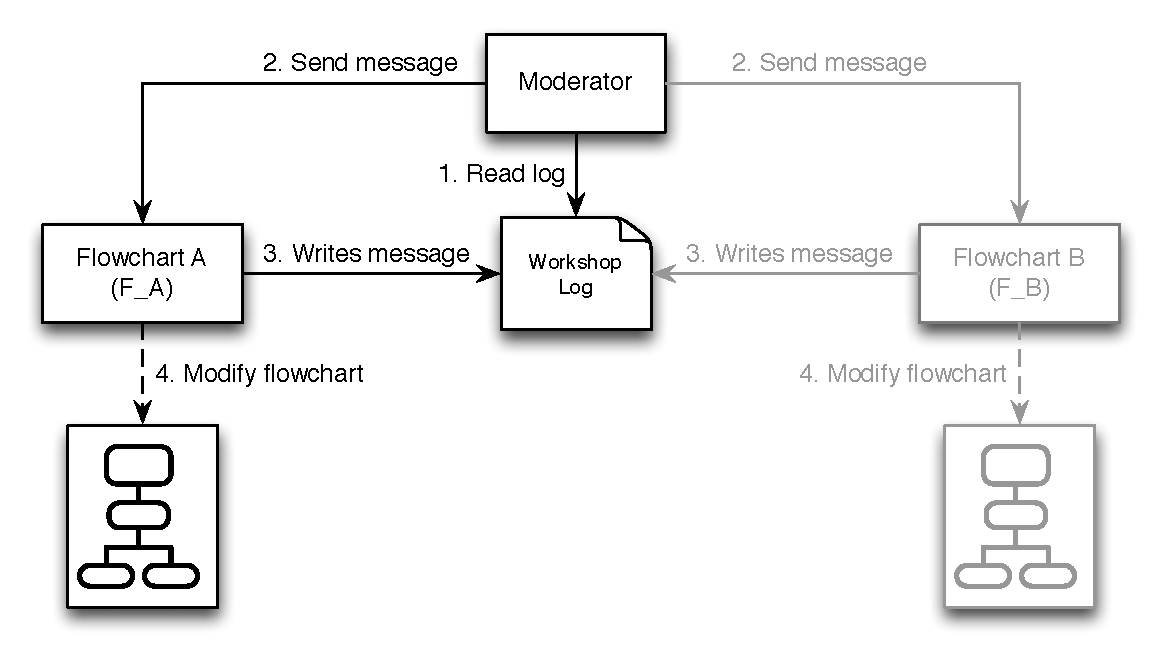
\includegraphics[width=\columnwidth]{figures/Schema}
\end{center}
\caption{Schematic diagram for a workshop built in the FloWr system\label{fig:workshop_schematic}}
\end{figure}

Keeping in mind the current limitations of FloWr -- no looping or conditionals, only running one flowchart at a time and in one direction -- a {\em conversation} between ProcessNodes or flowcharts is not immediately feasible.  Figure \ref{fig:workshop_schematic} represents a hypothetical design in which a Workshop could take place with a minimally-altered version of FloWr. As shown in Figure \ref{fig:workshop_schematic}, each participant in the Workshop would be represented by a single node. One of these nodes is a {\em moderator} in charge of dictating the interaction between the participants of the Workshop, while the rest represent {\em flowcharts} that have the ability to modify their own connections according to the discussions from the Workshop -- this can be achieved by exploiting the scripting mechanism of FloWr and dynamically loading the new structure of the flowchart. Moreover, a shared \emph{log} would contain the history of the messages exchanged during the Workshop and a queue of messages waiting to be delivered. We define four different types of messages that can be exchanged:
\begin{itemize}
% \item {\bf\em advertisement} of the overall capabilities of a participant.
\item {\bf\em comments} about specific elements of a poem, or more general appreciations of it.
\item {\bf\em questions} about specific details of a participant's capabilities; for instance, the questions can vary from simple requests of sources of information (e.g. files, input from another node, which resources a flowchart uses, etc.) to process-specific details (e.g. current conditions, purpose, other outstanding questions, etc.)
\item {\bf\em answers} would be associated to previous questions and may contain simple text such as an url for the source of information, or a piece of script representing a node used by a flowchart.
\item {\bf\em suggestions} are changes proposed by one participant to another. Similar to the answer, this can be as simple as suggesting the change of an information source, or more complex as suggesting the replacement of a node for an alternative node.
\end{itemize}

A Workshop session follows this communication protocol:
\begin{enumerate}
\item The moderator initialises an empty log and sends a message to the flowcharts to indicate that the session has started. 
\item The flowcharts start writing messages in the log.
\item The moderator checks the current state of the workshop by reading the log. \label{step:loop}
\item The moderator selects the next message in the queue and pass it to the target flowchart. 
\item The flowchart reads the message and acts accordingly by either (i) modifying its connections or (ii) sending a message back; i.e. writes in the log. 
\item Step \ref{step:loop} is repeated until no further message are left in the queue.
\end{enumerate}

% This protocol rises the following questions: from the suggestions received (i) which one is the best option?  (ii) how many options do we listen to before we even try to make a decision?   

\paragraph{Example.}
Figure \ref{poetryGeneratorFlowchart} shows the poetry generator flowchart that generates the poem about the ``demon dog'' presented above. The flowchart uses two linguistic resources: ConceptNet \cite{ConceptNet}, a semantic network of common knowledge, and Disco \cite{Disco}, a semantic similarity words retrieval system. Let us assume the human critic $\mathbf{A}$ has access to the system through a ``UI flowchart'' like a Read-Eval-Print Loop (REPL), and the poetry generator $\mathbf{B}$ is mainly concerned with maintaining a generative flowchart like the one shown in the figure. The following exchange of messages can occur:

\begin{enumerate}
\item \textbf{Comment from participant $\mathbf{A}$ to participant $\mathbf{B}$}: {\em The words ``lonely encounter'' and ``elusive ruler'' in lines 2 and 3 are generalised and imprecise}.
\item \textbf{Question from participant $\mathbf{B}$ to participant $\mathbf{A}$}: {\em I identify the processes {\em Disco3} and {\em Disco4} as the source of the problem. Can you suggest an alternative to Disco?} 
\item \textbf{Suggestions from participant $\mathbf{A}$ to participant $\mathbf{B}$}: {\em Use WordNet or the Historical Thesaurus to find more expressive and specific terms for the core concepts in the poem; try to link the core concepts together by chaining together related concepts in ConceptNet or WordNet.}%\footnote{\url{http://wordnet.princeton.edu/}}\textsuperscript{,}\footnote{\url{http://historicalthesaurus.arts.gla.ac.uk/}}
\item \textbf{Action executed by participant $\mathbf{B}$}: Receives suggestions, creates several alternative versions of the script, executes them and decides which one is most coherent and which conveys a sense of narrative.
\end{enumerate}

\noindent From this exchange, the computer might learn (without ever being explicitly told) that expressive terms and narratives are related, and it might find a way to produce coherent poems with a narrative structure.

\paragraph{Remark.}
Since the computer has source code instead of a brain, we can use it to do control studies with process.  However, in general source code does not completely determine process: contextual effects are what make an experiment an experiment.  As described in \cite{cook2013mechanics}, code does often include hints about context.  This is related to our theme of embedding process within an artefact.
%
In this connection, one extension to FloWr that would help to facilitate dialogue between flowcharts would be to add machine-readable \emph{commentary} to ProcessNodes.  Commentaries would label a node's inputs and outputs, describe its basic purpose, and providing information about procedure, conditional behaviour, mappings between processes and elements of the poem (like the mapping between Disco3 and ``lonely encounter''). 
% This would enable basic procedural communication between flowcharts and would also allow the system to identify where to apply suggestions for new versions of a flowchart as suggested in a workshop session. 

\begin{figure}[t]
\begin{center}
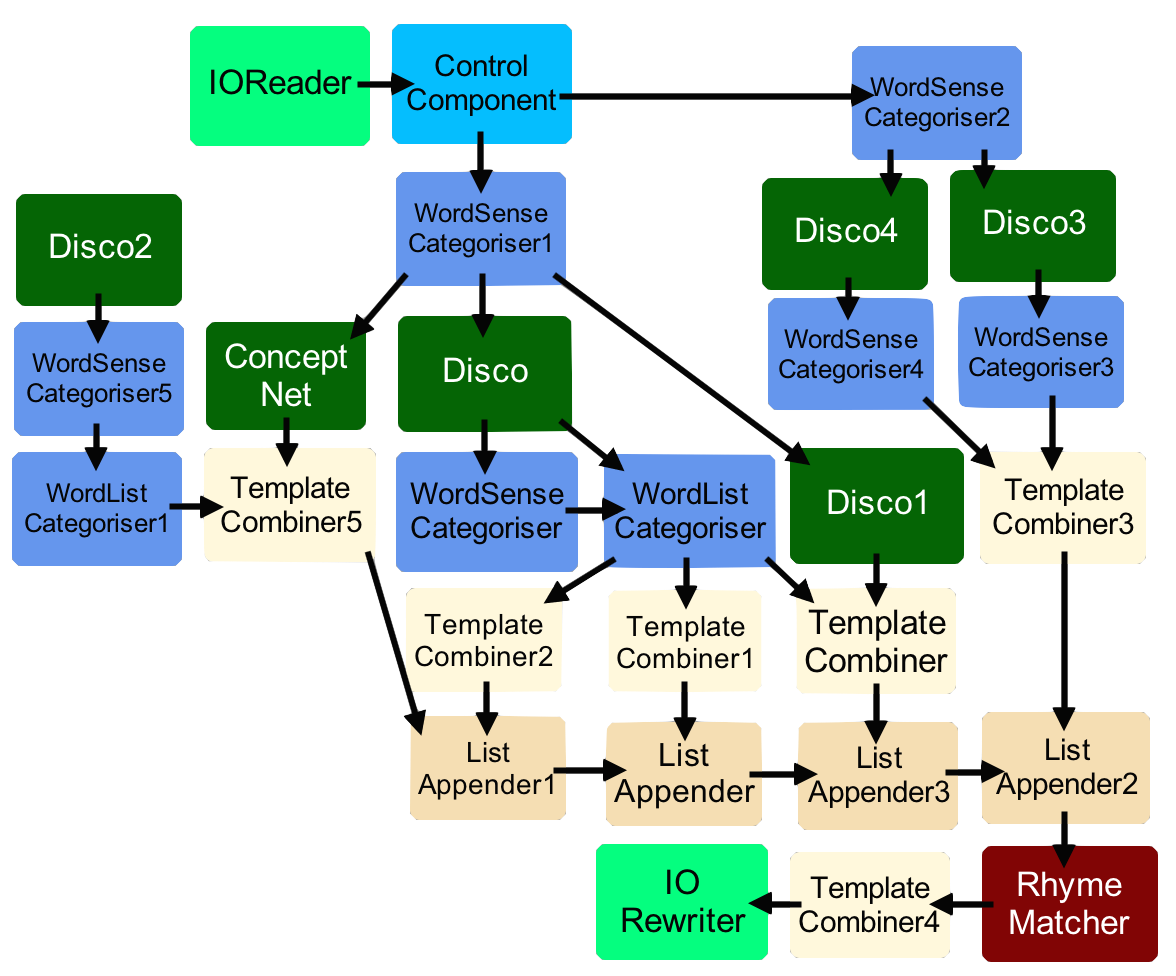
\includegraphics[width=\columnwidth]{./figures/PoemsFlowchart.png}
\caption{The flowchart that generated the ``demon dog'' poem}
\label{poetryGeneratorFlowchart}
\end{center}
\end{figure}

\paragraph{Down the garden path?}
Altered versions of a flowchart \cite{charnley2014flowr} can be seen as parallel solutions that could be executed and compared on a population basis with respect to some pre-specified metrics in order to make an informed decision on which suggestion(s) to follow, as hinted in the last step of the example.  In \cite{colton-assessingprogress} we explored the related idea of modelling system progress over time.  Learning new rules contextually would offer one clear measure of progress.  While these features sound good, we caution the reader that FloWr is still a research prototype, and considerable work would be required to realise the ideas we've described in FloWr or any other platform we're aware of.

%%% Local Variables: 
%%% mode: latex
%%% TeX-master: "mathsICCC"
%%% End: 

%% \section{Evaluation and Outlook}
\label{sec:eval}

Joe et al.

%%% Local Variables: 
%%% mode: latex
%%% TeX-master: "mathsICCC"
%%% End: 

%% \section{Conclusions}
\label{sec:conc}

We have made the case for dialogicity in CC and in CC research,
building on a comparison of different ways to read poems, and
considering the potential of an existing software system to support
dialogue at various levels.

Our requirements for communication points to the need for program
elements to be able to learn and adapt.  Genetic programming
\cite{koza1992genetic} and related methods offer a certain precedent
for this way of working.

The current paper has focused on more global concerns.  The current
FloWr ``ecosystem'' focuses on features like user interface ease for
human programmers, plus reusability of modules.  The next steps should
involve an agent-based redesign.  We have sketched related work in
Section \ref{sec:background}.  Off-the-shelf open source software
exists to support some relevant basic features.

However, the question of \emph{context} has not been adequately
addressed either in CC or in mainstream programming.  While we do not
agree with interpretations of artwork that macro-reductionistic in the
sense that ``the environment determines the artwork'' nevertheless
there are important contextual effects \cite{geertz1976art}, and
artwork generally involves an engagement with context.
Philosophically this situates the work in the realms of
\emph{pragmatics} \cite{sep-pragmatics} and \emph{metalinguistics}
\cite{gombert1994development}.  Practically speaking, the questions
relate to building sophistication in the specific ``metalanguage'' of
programming.  The programming tasks involved are not necessarily ends
in themselves, however, but oriented, in the first place towards
building better artefacts.  These too have a goal, which (at least in
a simple case) is to communicate.

The graphical programming environment that shipped with the 1984 robot
simulation game ChipWits, not taken seriously as a competitor to
FloWr, does nevertheless have some useful programming facilities, like
the ability to loop and run different paths in the flowchart depending
on conditions, and the ability for one flowchart to reference another
one, as with spreadsheets.  However, it does not have the ability to
self-program, which is the essence of the proposal for FloWr.  The
ability to generate-and-check (using a population-based mechanism) and
more importantly, the ability to learn over time (as we explored from
a formal perspective in \cite{colton-assessingprogress}) are two other
features that should come standard in future versions of FloWr.  We
want to be able to take account of the abundance of available
information, to introduce ``noise'', and fully take account of the
existing ``framing'' in relationship to the context/situation.

Although social creativity has been explored in CC, it tends to be an
exception rather than the rule.  In future work, we'd like to be able
to say ``We've done it!'' although to develop a concrete proof of
concept we will have to focus on a few simple metrics (like
musicality).

There is also a ``social engineering'' component to this paper, hoping
to motivate a new approach to research evaluation in CC.  Between the
kind of design research carried out in this paper and a large-scale
double-blind study that would ``prove'' the superiority of a social
approach is something more contextual, involving the actual practices
and abilities of participants
\cite[pp. 167--185]{seikkula2006dialogical}.  We sketched an approach
to the evaluation of poems, but similar thinking can help develop an
evaluation of programs.  The question of how much architecture should
be shared in the CC community: do we need a shared ``CCyc'' platform,
or should we ``let a hundred flowers bloom''?  One moderate approach
would be to revive the \emph{floral games} of the troubadours.

%%% Local Variables: 
%%% mode: latex
%%% TeX-master: "mathsICCC"
%%% End: 


%% \section*{Acknowledgements} \label{sec:acknowledgements}
%% This research has been supported by EPSRC grants EP/L00206X and
%% EP/J004049, and the Future and Emerging Technologies (FET) programme
%% within the Seventh Framework Programme for Research of the European
%% Commission, under FET-Open Grant numbers: 611553 (COINVENT) and 611560
%% (WHIM).

\printbibliography

\end{document}
